\section{Results}

\subsection{Harder arithmetic supports causal masking}

Table~\ref{tab:harder-multiseed} shows the 500-example harder arithmetic evaluation after training on 2,000 preference pairs over three seeds. Vanilla DPO is consistently harmful. Prefix-masked and first-error-only DPO are much stronger. \cmdpo{} is best on average, but its margin over first-error-only DPO is small.

\begin{table}[t]
\caption{Harder arithmetic eval500 after harder2000 training. Mean and standard deviation are over three seeds.}
\label{tab:harder-multiseed}
\begin{center}
\begin{tabular}{lcc}
\toprule
Model & Accuracy & Std. \\
\midrule
Base & 0.410 & -- \\
Vanilla DPO & 0.253 & 0.054 \\
Prefix-masked DPO & 0.365 & 0.012 \\
First-error-only DPO & 0.427 & 0.016 \\
\cmdpo{} & \textbf{0.433} & 0.011 \\
\bottomrule
\end{tabular}
\end{center}
\end{table}

This result supports the central causal-masking claim: uniformly penalizing rejected reasoning is unsafe, and protecting pre-error reasoning substantially improves behavior. It does not, by itself, prove that suffix decay is much better than simply training on the first erroneous step.

\subsection{Ablation: prefix protection versus suffix decay}

The four variants decompose the effect of causal masking. Vanilla DPO has no prefix protection and drops from a base accuracy of $0.410$ to $0.253$. Prefix-masked DPO changes only the pre-error prefix weights and recovers much of the lost performance, reaching $0.365$. First-error-only DPO removes suffix pressure entirely and reaches $0.427$. \cmdpo{} keeps a decayed suffix penalty and reaches $0.433$.

This pattern supports a clear primary conclusion and a cautious secondary one. The primary conclusion is that prefix protection is responsible for the largest improvement over vanilla DPO. The secondary conclusion is that suffix decay can help in the controlled setting, but the observed gain over first-error-only DPO is small relative to the current scale of the experiments.

\subsection{Suffix schedule controls the error--suffix tradeoff}

Table~\ref{tab:gamma-likelihood} reports a deterministic likelihood probe after harder2000 training. The endpoints correspond to first-error-only DPO ($\gamma=0$) and prefix-masked DPO ($\gamma=1$). All settings strongly increase the likelihood of pre-error prefixes, confirming that causal masks protect correct rejected prefixes. Increasing $\gamma$ makes the first-error penalty stronger, but it also increasingly penalizes post-error suffix tokens. The $\gamma=0.75$ setting gives the strongest first-error suppression among decayed schedules, while $\gamma=1$ behaves like full suffix penalty and heavily suppresses the suffix.

\begin{table}[t]
\caption{Harder2000 likelihood probe for \cmdpo{} suffix schedules. Entries are post-training minus pre-training masked log-likelihood changes on rejected spans. Higher prefix delta means better prefix retention; more negative error delta means stronger first-error suppression.}
\label{tab:gamma-likelihood}
\begin{center}
\begin{tabular}{lrrrr}
\toprule
Schedule & Prefix $\Delta$ & Error $\Delta$ & Suffix $\Delta$ & Mask $\Delta$ \\
\midrule
$\gamma=0$ & 35.112 & -18.082 & 17.304 & -15.091 \\
$\gamma=0.25$ & 35.234 & -20.470 & 16.688 & -17.658 \\
$\gamma=0.5$ & \textbf{35.320} & -20.866 & 15.317 & -18.392 \\
$\gamma=0.75$ & 35.254 & -23.838 & 11.550 & -22.246 \\
$\gamma=1$ & 35.102 & \textbf{-27.394} & -44.424 & \textbf{-35.863} \\
\bottomrule
\end{tabular}
\end{center}
\end{table}

\begin{figure}[t]
\centering
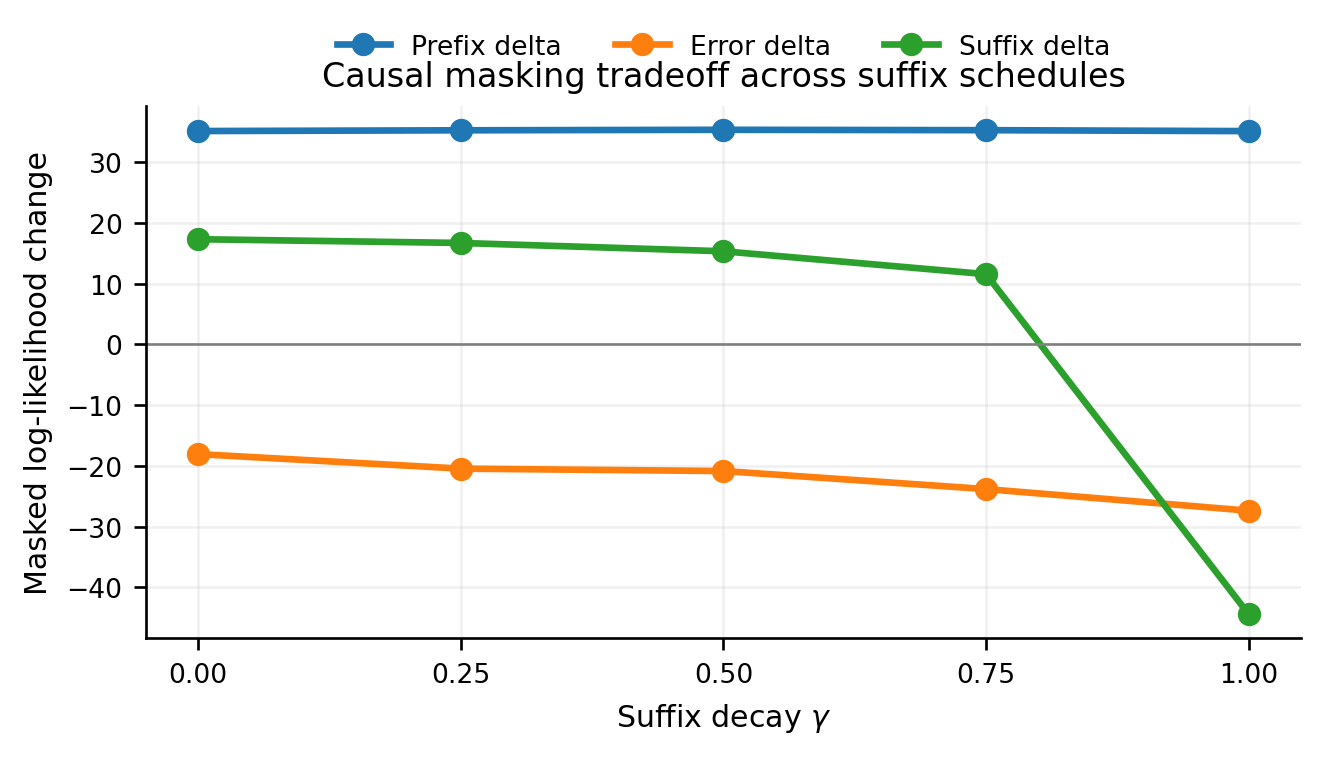
\includegraphics[width=\linewidth]{figures/gamma_sweep.png}
\caption{Suffix-schedule tradeoff on harder2000. Prefix retention stays stable, while stronger suffix decay increasingly suppresses the first error and eventually flips the suffix behavior at $\gamma=1$.}
\label{fig:gamma-sweep}
\end{figure}

This ablation clarifies why suffix decay should be treated as a schedule rather than a single fixed claim. Small and moderate $\gamma$ values preserve prefix likelihood and suppress the first error without aggressively suppressing inherited suffix text. Large $\gamma$ values more closely resemble prefix-masked DPO: they apply strong pressure to all post-error tokens, which can be useful for error suppression but risks treating consequence steps as independently wrong.

\subsection{Diagnostics support the mechanism}

Additional controls in Appendix~\ref{app:diagnostics} test alternative explanations. A truncated-rejected baseline suppresses first errors but still harms correct prefixes, so the gain is not merely due to shorter rejected responses. Normalizing the rejected-side mask or uniformly down-weighting all rejected tokens preserves prefix likelihood but fails to suppress the localized error, indicating that mask structure and penalty mass are not interchangeable. Localization-noise controls show that shifting the first-error index earlier harms prefixes, while shifting it later or randomly corrupting 25\% of labels weakens true-error suppression.

\subsection{GSM8K pilots are mixed}

Table~\ref{tab:gsm8k-pilots} summarizes the GSM8K-style pilots on a 100-example evaluation set. As localization and filtering improve, all trained variants can beat the base model. However, \cmdpo{} does not dominate. Prefix-masked DPO is best in the 109-example high-quality setting, while first-error-only is best in the more-candidates setting.

\begin{table}[t]
\caption{GSM8K-style eval100. Entries are correct out of 100.}
\label{tab:gsm8k-pilots}
\begin{center}
\begin{tabular}{lccccc}
\toprule
Training data & Base & Vanilla & Prefix & First-error & \cmdpo{} \\
\midrule
Cheap localizer, 49 rows & 16 & 19 & \textbf{22} & 21 & 20 \\
API judge, 49 rows & 16 & 18 & \textbf{25} & 23 & 20 \\
API judge HQ, 109 rows & 16 & 25 & \textbf{29} & 28 & 28 \\
More-candidates HQ, 87 rows & 16 & 22 & 25 & \textbf{28} & 27 \\
\bottomrule
\end{tabular}
\end{center}
\end{table}

Localization and filtering diagnostics are reported in Appendix~\ref{app:gsm8k-diagnostics}. The robust conclusion is that prefix protection matters. The suffix-decay component of \cmdpo{} remains plausible on controlled arithmetic, but the GSM8K pilots do not yet establish it as a reliable additional improvement.

\subsection{A larger 1.5B run is mixed}

To check whether the mechanism persists at a larger model scale, we trained Qwen2.5-1.5B-Instruct on 1,000 harder arithmetic preference pairs and evaluated on a 500-example harder arithmetic set. The generation metric is mixed: vanilla DPO achieves the highest accuracy on this particular run, while \cmdpo{} remains far above the base model but below vanilla. The likelihood probe still shows the same structural separation between prefix protection and rejected-side suppression.

\begin{table}[t]
\caption{Harder1000 training with Qwen2.5-1.5B-Instruct. Accuracy is evaluated on harder eval500. Likelihood entries are post-training minus pre-training masked log-likelihood changes on the harder1000 training set.}
\label{tab:qwen15b}
\begin{center}
\begin{tabular}{lcc}
\toprule
Model & Accuracy & Prefix $\Delta$ / Error $\Delta$ \\
\midrule
Base & 0.118 & -- \\
Vanilla DPO & 0.498 & -16.626 / -36.310 \\
\cmdpo{} & 0.224 & 21.352 / -17.321 \\
\bottomrule
\end{tabular}
\end{center}
\end{table}

\begin{figure}[t]
\centering
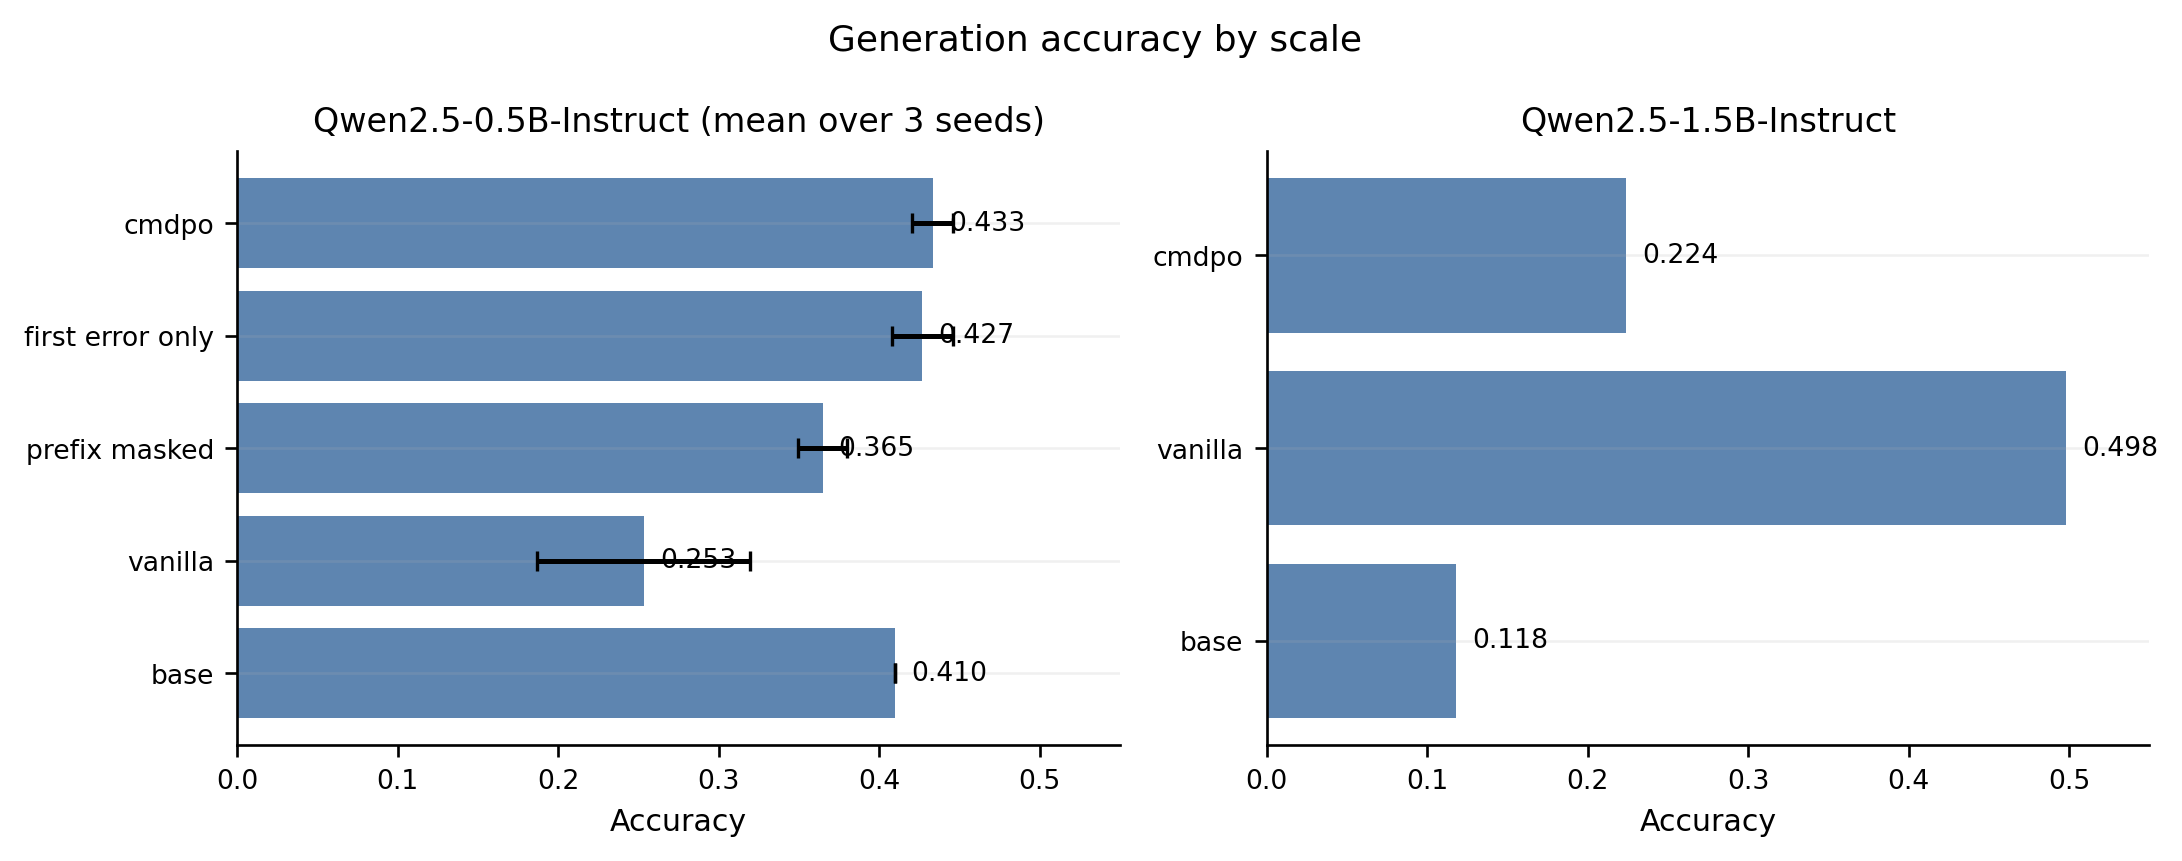
\includegraphics[width=\linewidth]{figures/scale_accuracy.png}
\caption{Accuracy by scale. The 0.5B setting uses the mean over three seeds on harder2000; the 1.5B setting is the single harder1000 run. The larger model changes the raw-accuracy ranking, so we treat the mechanism probe as the more stable evidence.}
\label{fig:scale-accuracy}
\end{figure}

This larger run does not support a simple stronger-is-better story for \cmdpo{}. It does, however, reinforce the paper's narrower claim: when rejected traces contain correct prefixes, vanilla DPO can suppress them aggressively, while causal masking preserves them more explicitly.
